\documentclass[12pt,preprint]{aastex}
\usepackage{graphicx}


%%%%%%%%%%%%%%%%%%%%%%%%%%%%%%%%%%%%%%%%%%%%%%%%%%%%
%%% author-defined commands
\newcommand\x         {\hbox{$\times$}}
\newcommand\othername {\hbox{$\dots$}}
\def\eq#1{\begin{equation} #1 \end{equation}}
\def\eqarray#1{\begin{eqnarray} #1 \end{eqnarray}}
\def\eqarraylet#1{\begin{mathletters}\begin{eqnarray} #1 %
                  \end{eqnarray}\end{mathletters}}
\def\mic              {\hbox{$\mu{\rm m}$}}
\def\about            {\hbox{$\sim$}}
\def\Mo               {\hbox{$M_{\odot}$}}
\def\Lo               {\hbox{$L_{\odot}$}}
\def\comm#1           {{\tt (COMMENT: #1)}}
%%%%%%%%%%%%%%%%%%%%%%%%%%%%%%%%%%%%%%%%%%%%%%%%%%%%


\begin{document}

\title{Level 2 Photometric Calibration for the LSST Survey}

\author{
Lynne Jones, David Burke, \v{Z}eljko Ivezi\'{c}, and the Photometric Calibration Team
}

%\begin{abstract}
%\end{abstract}


\section{Introduction}


Two levels of LSST photometric calibration will be carried out at
differing cadences and with differing performance targets. A nightly
data calibration based on the best available set of prior calibrated
observations will provide “best-effort” precision and accuracy. This
calibration will be used for quality assurance, generation of alerts
to transients, and other quantities appropriate for Level 1 Data
Products.  A more complete analysis will recalibrate the data
accumulated by the survey at periodic “Data Release” dates (Level 2 in
LSST data management terminology.)  It is this repeated calibration of
the accumulated survey that will be held to the survey requirements
for photometric repeatability, uniformity, and accuracy.  This
document describes the calibration requirements and processes for the
Level 2 photometric calibration.

\section{Photometric Requirements}

The LSST Science Requirements Document (SRD) specifies that the survey
must deliver photometry with the following characteristics:
\begin{enumerate}
\item{Repeatability of 5 millimags in $gri$, 7.5 millimags in $uzy$,
for bright unresolved sources.  This specifies the distribution of
random photometric errors ($\sigma$) and constrains both the
repeatability of extracting counts from images and the ability to
monitor (or model) the changes in normalized system response
($\phi$). It could be thought of as making the photometry of a single
source consistent over time. \label{repeatability_req}}
\item{Uniformity of 10 millimags in $grizy$, and up to 20 millimags in
$u$, again for bright unresolved sources. This places a constraint on
the stability of the photometric system across the sky and places an
upper limit on various systematic errors, such as a correlation of
internal photometric zero-point error with the position on a
sensor. This makes the photometry of many sources comparable over the
entire sky, which when combined with the previous requirements creates
a stable photometric system across the sky and over time, in a single
filter. \label{uniformity_req}}
\item{Band-to-band zero-point calibration for main sequence stars of 5
millimags for any color not involving $u$ band, 10 millimags for
colors constructed with $u$ band photometry. This constrains the upper
limit of the systematic error in the measurement of the system
throughput as a function of wavelength. This requirement ties
photometric measurements in different filters together, enabling
colors to be measured for sources with unknown SEDs or (for sources
with known SEDs) magnitudes in different filters to be directly
compared. \label{color_req}}
\item{Zero-point calibration with respect to an external system of 10
millimags. This requirement ties LSST internal photometry to a
physical scale, and places a constraint on the upper limit of the
systematic error in the measurement of the total system
throughput. This final step enables LSST photometry to be compared
with photometry from other telescopes using other photometric
systems. \label{abs_req}}
\end{enumerate}

Requirements \ref{repeatability_req} and \ref{uniformity_req} must be
met by compensating for changes in system sensitivity as a function of
time, location in the sky or focal plane, and result in a relative
calibration within a single filter. Requirements \ref{color_req}
and \ref{abs_req} require additional measurements of sources with
known colors and absolute magnitudes, where these additional
measurements result in a relative calibration from filter to filter as
well as an absolute physical scale for the overall system.

Only photometric measurements released as part of the data release
products (generated annually) will be held to the requirements
above. On a nightly timescale, photometric measurements needed for
alert generation, quality assurance, or other short-timescale data
products will be generated to ``best-effort'' precision and accuracy
using the best-available prior calibrated observations.

\section{Overview of the photometric calibration process}

The photometric requirements described above are a factor of 2 better
than those previously achieved by wide-field surveys operating on
primarily photometric nights. To reach the SRD level of precision using
observations taken under a wide variety of conditions (including
non-photometric nights) requires a new approach. This is possible by
gathering additional data on the wavelength dependence of the
throughput of the hardware system and the atmosphere and by leveraging
the multiple observations of many stars that LSST will
gather. Traditional photometric calibration uses a set of standard
stars, observed at a range of airmasses in between science
observations, to calculate zeropoint offsets and perhaps a single
color-dependent extinction term for the science images. Calibration of
LSST magnitudes to SRD levels, under conditions with up to XXX cloud
extinction, would require standard stars in every CCD of every
exposure: this standard star network is thus necesssarily defined as the
non-variable, isolated, bright stars observed within LSST itself. In
addition, when considering the possibility of $>1\%$ variations in the
filter bandpasses across the field of view and/or the strong effects
of water band absorption in the $y$ band, it becomes clear that LSST
must measure and correct for wavelength-dependent effects to a much
higher level than previous surveys. This section describes and motivates our
photometric calibration approach. 

Given $F_\nu(\lambda)$, the specific flux of an object {\it at
the top} of the atmosphere, at a position described by ($alt$,$az$),
the flux transmitted through the atmosphere to the telescope pupil is
\begin{equation}
\label{eqn:Fpupil}
   F_\nu^{pupil}(\lambda,alt,az,t) = F_\nu(\lambda) \, S^{atm}(\lambda,alt,az,t),
\end{equation}
where $S^{atm}(\lambda,alt,az)$ is the (dimensionless) probability that a photon of 
wavelength $\lambda$ makes it through the atmosphere,
\begin{equation}
\label{eqn:atmTau}
   S^{atm}(\lambda,alt,az,t)   = {\rm e}^{-\tau^{atm}(\lambda,alt,az,t)}.
\end{equation}
Here $\tau^{atm}(\lambda,alt,az)$ is the optical depth of the
atmospheric layer at wavelength $\lambda$ towards the position
($alt$,$az$).  Observational data show that $\tau^{atm}$'s dependency
on wavelength is slowly varying with time ($t$) (on the order of
5-10\% over an hour near the water bands) and position ($alt$,$az$)
(primarily a function of airmass, but additional variation on the
scale of tens of degrees can be detected due to water vapor
absorption) (LSST-5367?), under `typical' observing conditions.  
Clouds represent an additive gray (non-wavelength dependent)
contribution to $\tau^{atm}$ which can introduce a strong variation of
$\tau^{atm}$ on much smaller angular scales and short timescales (on
the order of 2-10\% of the total extinction at $1^{\circ}$ scales,
variable within minutes) (Ivezic2007). 

Note that while both $F_\nu(\lambda,t)$ and $\tau^{atm}(\lambda,alt,az,t)$ 
could vary more quickly than the standard LSST exposure time of 15
seconds, it is assumed here that all quantities are averaged over some
short exposure time and that $t$ indicates that the quantities could
vary from exposure to exposure. 

Given $F_\nu^{pupil}(\lambda,alt,az,t)$, the counts recorded at a
position within the field of view described by ($x$,$y$) can be
written as
\begin{equation}
\label{eqn:Fpupil2counts}
    C_b(alt,az,x,y,t) = C \, \int_0^\infty {F_\nu^{pupil}(\lambda,alt,az,t) \, S_b^{sys}(\lambda,x,y,t) \lambda^{-1}d\lambda}.
\end{equation}
Here, $S_b^{sys}(\lambda,x,y,t)$ is the (dimensionless) probability
that a photon will be converted into an ADU count, and the term
$\lambda^{-1}$ comes from the conversion of energy per unit frequency
into the number of photons per unit wavelength ($b=ugrizy$). The
dimensional conversion constant $C$ is
\begin{equation}
\label{eqn:Cconstant}
        C = {\pi D^2 \Delta t \over 4 g h }  
\end{equation}
where $D$ is the effective primary mirror diameter, $\Delta t$ is the
exposure time, $g$ is the gain of the readout electronics (number of
photoelectrons per ADU count, a number greater than one), and $h$ is
the Planck constant. The system response function,
$S_b^{sys}(\lambda,x,y)$, includes the effects of the mirror
reflectance, optics transmission and detector sensitivity. In general,
the wavelength-dependent variations in $S_b^{sys}$ change slowly; over
periods of months, the mirror reflectance and filter transmission will
degrade as their coatings age. There will likely also be a
wavelength-dependent spatial variation in $S_b^{atm}$ due to
irregularities in the filter material caused by production methods,
which will vary slowly from the center of the field of view to the
outer edges (Regnault REF). Spatial variations in $S_b^{sys}$ that are
independent of wavelength can occur more rapidly in time, on the
timescale of a day, and in spatial scale, on a pixel level. These
variations are caused by dust on the dewar window or filter or
detector sensitivity variations on the pixel-to-pixel scale, and can
be treated as wavelength-independent.
%A more rapid wavelength-dependent variation in
%detector sensitivity (especially at the very red wavelengths in the
%$y$ band) results from variations in the temperature of the detector,
%but with little or no spatial variation.

From equation~\ref{eqn:Fpupil2counts} and the paragraphs above, we can
see that the generation of counts $C_b(alt,az,x,y,t)$ from photons is
imprinted with many different kinds of effects, which have different
scales of variability over time ($t$), spatial scale ($alt$, $az$ or
$x$, $y$), and wavelength ($\lambda$), suggesting that it is
beneficial to separate these effects for calibration
purposes. This may be
seen more easily by introducing $\phi_b(\lambda,alt,az,x,y,t)$, the normalized system
response in a filter $b$ for a particular observation,
\begin{equation}
\label{eqn:PhiDef}
   \phi_b(\lambda,alt,az,x,y,t) = {
     {S^{atm}(\lambda,alt,az,t) S_b^{sys}(\lambda,x,y,t) \slash
       \lambda} \over
     \int_0^\infty { {S^{atm}(\lambda,alt,az,t) 
         S_b^{sys}(\lambda,x,y,t) \slash \lambda} \,d\lambda}}.
\end{equation}
By definition, $\int_0^\infty {\phi_b(\lambda) d\lambda}=1$.  From
Equations~\ref{eqn:Fpupil} and~\ref{eqn:Fpupil2counts}, we can then
recast the counts measured as
\begin{eqnarray}
\label{eqn:fullcounts}
C_b(alt,az,x,y,t) & = & C \, \int_0^\infty {F_\nu(\lambda,t)
  S_b^{atm}(\lambda,alt,az,t) \, S_b^{sys}(\lambda,x,y,t)
  \lambda^{-1}d\lambda} \\
&= & C'(alt,az,x,y,t) \,
     \int_0^\infty {F_\nu(\lambda,t)\phi_b(\lambda,alt,az,x,y,t)
       d\lambda} 
\end{eqnarray}
where $C'(alt,az,x,y,t)$ is a gray normalization value that depends
on the total system throughput. We can also introduce
$\phi_b^{std}(\lambda)$, a `standardized' bandpass, so
\begin{eqnarray}
C_b(alt,az,x,y,t) & = & C'(alt,az,x,y,t)
\left( {\int_0^\infty {F_\nu(\lambda,t)\phi_b^{obs}(\lambda,alt,az,x,y,t) d\lambda} \over 
\int_0^\infty {F_\nu(\lambda,t)\phi_b^{std}(\lambda) d\lambda}} 
\right) \int_0^\infty {F_\nu(\lambda,t)\phi_b^{std}(\lambda)  d\lambda}
\nonumber \\ 
& = & C'(alt,az,x,y,t) \, K'(F_\nu(\lambda,t),
\phi_b^{obs}(\lambda,alt,az,x,y,t) 
\int_0^\infty {F_\nu(\lambda,t)\phi_b^{std}(\lambda)  d\lambda} 
\end{eqnarray}
where $K'(F_\nu, \phi_b^{obs})$ is a wavelength and source SED
dependent value that depends on the shape of the system throughput,
but not on its normalization. The values 
\begin{equation}
\label{eqn:defnatmags}
%m_{nat}  & = &-2.5 log_{10} \left( {C_b(alt,az,x,y,t) \over C'(alt,az,x,y,t) \, K'(F_\nu(\lambda,t),
%\phi_b^{obs}(\lambda,alt,az,x,y,t)} \right) \nonumber \\
 m_b^{nat} =  -2.5 log_{10} (\int_0^\infty {F_\nu(\lambda,t)\phi_b^{std}(\lambda)  d\lambda})
\end{equation}
represent `natural magnitudes', directly comparable from
one observation to another although they are not tied to an external
physical scale. The wavelength-dependent effects tied into
$K'(F_\nu(\lambda,t), \phi_b^{obs}(\lambda,alt,az,x,y,t))$ can be
considered variations in the {\it shape} of the bandpass; the
gray-scale effects tied into $C'(alt,az,x,y,t)$ are variations in the
{\it normalization} of the bandpass.  Furthermore, variations in the
normalization of the bandpass caused by the {\it hardware} system can be separated from the
variations in the bandpass caused by the {\it atmosphere}, and
measured with different methods, splitting
$C'(alt,az,x,y,t)$ into $C''(alt,az,t)$ and $C''(x,y,t)$ portions. It
is more difficult for $K'(F_\nu, \phi_b^{obs})$, as the atmosphere and
hardware effects on the total counts are not truly independent,
however the underlying wavelength-dependent variations in $S_b^{sys}$
and $S^{atm}$ {\it are} independent and can be measured separately and
only applied to the measured counts as a combined correction. 

Let us first consider all variations in $S_b^{sys}(\lambda,x,y,t)$, as
these vary on timescales quite different from
$S^{atm}(\lambda,alt,az,t)$.  We can further divide and correct the
measured counts for variations in $S_b^{sys}(\lambda,x,y,t)$, the
throughput in the hardware system, as follows. Using a dome-screen
system that is capable of producing light at a range of individual
wavelengths (the ``stubbsometer''), we can measure the sensitivity of
the mirror/lens/filter/detector system as a function of $x$,$y$ at
each wavelength, producing a series of `narrow band flat
fields'. While it would be possible to use these as a standard flat
field (after choosing a particular method to combine the measurements
at different wavelengths), it is not possible to generate all the
necessary narrow band flats each night; scanning through all 6 filters
at 1nm intervals requires tens of hours. However, since the
wavelength-dependent effects are expected to vary slowly over time, we
can instead plan to only produce narrow band flat fields every 30
days. Using standard white-light flat fields for each filter acquired
at the start and end of observing on each night, we can also correct
for the much more rapidly changing wavelength-independent effects
(dust accumulation, pixel-to-pixel sensitivity variations, etc.) that
occur primarily on scales smaller than the PSF. The images are
corrected for gray-scale effects with the white-light flat field, and
also corrected for the wavelength-dependent effects in system
throughput measured from the narrow band flats.

Next, considering $S_b^{atm}(\lambda,alt,az,t)$, we again
separate the wavelength-dependent variations, which occur over
spatial scales larger than the field of view and several minute timescales, from the gray
variations due to clouds, which occur over much smaller spatial and
time scales. By using an auxiliary telescope equipped with a
spectroscope to examine bright stars near the main telescope's field
of view with known spectral energy
distributions, we can measure the absorption lines in
the atmosphere every 5--10 minutes. These observations are used as
constraints for MODTRAN atmospheric models, generating simpler
representations of the atmospheric throughput which can be
interpolated to provide models of the wavelength-dependence of
$S_b^{atm}(\lambda,alt,az,t)$ in each observation. In order to correct
for the higher frequency gray-scale variations in $S_b^{atm}$, we must
use the observations of the stars themselves; because we have many repeat
observations of many stars, we can use a `self-calibration' procedure
similar to the ubercal method used with SDSS Stripe 82 data
(Padmanabhan REF). By selecting non-variable, main-sequence stars
from each observation, then minimizing the least-squares differences
between these observations, we can determine the extinction due to
clouds within each chip, then apply this extinction to all other
photometric measurements from the same observation. 

To summarize: pixel-to-pixel gray sensitivity variations are corrected
using white-light flat fields, wavelength-dependent
variations of the hardware system across the field of view are
corrected with narrow band flats generated by the ``stubbsometer''
dome screen, wavelength-dependent variations due to the atmosphere are
corrected with MODTRAN models generated using the auxiliary telescope,
and gray variations on the scale of a CCD due to clouds are corrected
using self-calibration. Each of these steps are necessary to achieve
0.5\% precision in repeat photometry and 1\% precision in photometric
stability across the sky (requirements \ref{repeatability_req} and
\ref{uniformity_req} ). These can be conceptually related to the natural magnitudes
(Eqn~\ref{eqn:defnatmags})  as 
\begin{eqnarray}
\label{eqn:defnatmags2}
m_b^{nat} & = &-2.5 \, log_{10} \, (C_{b, raw}(alt,az,x,y,t))  \\ 
 & & +\, \delta z_b^{ff}(x,y,t) + \delta k_b^{ff}(x,y,SED,t)  \nonumber \\  
 & &+\, \delta z_b^{selfcalib}(alt,az,t)  + \delta k_b^{atm}(alt,az,SED,t)  \nonumber
\end{eqnarray}
where the raw counts from the object in the image are translated to an
internally consistent magnitude through corrections from the flat
field, stubbsometer, atmospheric models and self-calibration
procedures. The wavelength-dependent zeropoint offsets, $\delta k$, are
equivalent to correcting the {\it shape} of the bandpass in each
filter to a `standard' bandpass and their values (for a particular object) 
depend on the spectral energy distribution of that object (and in detail, $\delta k_{ff}$ is actually
dependent on $\delta k_{atm}$). The wavelength-indepedent
zeropoint offsets, $\delta z$, are equivalent to
correcting the {\it normalization} of the bandpass to a common
standard.  The natural magnitudes are not, however, tied to an
external physical scale, nor are measurements in one filter tied to
measurements in another filter (requirements \ref{color_req} and
\ref{abs_req}).

To fulfill these last two requirements a further set of measurements
are needed. In all filters, a set of objects with a well-known
spectral type (such as main sequence stars or white dwarfs, preferably
with direct observations of the SED of the specific object) must be
observed and calibrated, in individual filters, as above. The prior
knowledge of each SED is combined with the `standard bandpass' shape
to generate synthetic color photometry. These synthetic colors are
then compared with the calibrated natural magnitudes from
Eqn~\ref{eqn:defnatmags} to calculate $\Delta_{b-r}$, the corrections
needed to tie measurements in each filter together (referenced to $r$
band).  At this point, only one final measurement is necessary to tie
the entire system to an external physical scale: an $r$ band LSST
natural magnitude measurement of an absolutely calibrated source on a
photometric night. Although in theory these last two steps could be
done with a single externally calibrated object, on a single
photometric night, a larger set of external reference objects spread
throughout the sky will be used to reduce systematic errors. This then
produces a final magnitude, 
\begin{equation}
\label{eqn:extmags}
m_b^{ext} = m_b^{nat}  + \Delta_{b-r} + \Delta_r
\end{equation}
which can be compared to physical flux scales. Placing our photometric
measurements on a standardized internal system and then tying this
internal system to an external flux scale, allows a separation
of the errors which arise from internal calibration vs. external
calibration. 

Using the calibration methods described to this point, it is possible
to translate counts from a particular object into photons above the
atmosphere; unfortunately extracting the counts from a particular
source in an image adds additional complications that are worth
mentioning in this overview. In addition to the counts from a
particular object of interest, in each pixel there are also photons
from the sky background, stray or scattered light from outside the
field of view, and stray light in each pixel from other sources
in the image (ghosting). These effects can be removed when conducting
the photometry measurements in the image, by calculating and removing
the local background, but this process must be included in the error
budget.

More problematic is that these effects (ghosting, stray/scattered
light), plus the effects of the variation of pixel scale across the
image, are present in the flat field as well. Since the flat field is
necessarily divided into each science image to remove pixel-to-pixel
sensitivity variations, this has the side-effect of encoding the
effect of ghosting and stray/scattered light {\it in the flat field}
into the science images. The pixel scale variation from the center of
the field of view to the outer edges of the field of view is another
problem which arises due to the flat field processing; although the
light from an individual object remains the same whether it is in the
center of the field of view or at the edge, the amount of sky
background (or dome illumination) observed in the images varies.
Creating an image where the background is `flat' across the image
means that the counts from the astronomical objects have been altered.
Thus, a further correction to the flat field - usually called
an `illumination correction' - must be made, to remove the effects of
stray and scattered light, ghosting, and the pixel scale variation
from the flat field. This illumination correction will be generated by
combining the measurements of the system throughput from the dome
screen (in white-light and narrow band flats), with raster-scans of
bright, dense star fields obtained through specialized observing
sequences, and measurements of the ghost patterns at each wavelength
caused by light at various locations within the field of view obtained
with the ``camera calibration optical bench'' (CCOB).  The flat field
corrections described in Eqn~\ref{eqn:defnatmags2} should be considered to
come from this illumination-corrected flat field; it is possible (as
the ghosting pattern is wavelength-dependent) that this illumination
correction may have some wavelength dependence. 
 
\subsection{Why not use self-calibration alone?}

One might also ask why all of the steps in the overview above
(white-light flatfields, narrow band dome flats, an illumination
correction, and models from measurements of atmospheric absorption)
are necessary, as in theory the self-calibration could account for
these corrections in addition to the effects of clouds. In practice,
however, the minimization between observed and predicted magnitudes
that occurs during self-calibration has limitations, which will be
further detailed in section~\ref{sec:selfcalib}.  In particular, the
minimization algorithm can fail to converge to the required level of
precision if the input magnitudes are sufficiently far from the model
predicted values.  Color terms in particular can be problematic. For
example, an uncorrected and unknown color term arising from a 2.5\%
radial gradient in the wavelength of the filter would cause
self-calibration to fail to converge to the 0.5\% photometric
repeatability requirement with 2 years of simulated data. Another
limitation is that the self-calibration cannot possibly correct for
any effects smaller than the PSF, not will it correct for
effects on scales smaller than a few times the mean separation of
calibration stars. Thus it is necessary to correct the photometric
measurements as much as possible before self-calibration using the
white-light (illumination-corrected) flatfields, the narrow band dome
flats, and the atmospheric absorption model.

Adding these corrections directly at the image level as much as
possible (rather than as a series of zeropoint offsets) will also
benefit photometric precision for extended objects. This is
particularly true for the illumination correction.

\section{Details of the internal calibration process}

The next sections describe further details of the calibration process
and how each correction is measured, calculated and applied. These
procedures are applied to each filter independently. The end
result of the internal calibration process is a set of natural
magnitudes, $m_b^{nat}$, measured for each object in each visit, as
well as a record of $\phi^{atm}(\lambda,alt,az,t)$,
$\phi_b^{sys}(\lambda,x,y,t)$, the flat field applied, the
zeropoint offset calculated for cloud extinction and the spectral
energy distribution assumed for the object to calculate $m_b^{nat}$.

\subsection{Measurement of the system transmission}

Variations in measured counts which results from changes in the hardware
(system) transmission function, $S_b^{sys}(\lambda,x,y,t)$, are corrected
through a `synthetic' flat field created from a combination of
narrow-band flat fields, white-light flat fields and an illumination correction.
Wavelength-dependent spatial changes are measured directly through the
narrow band flats combined with the illumination correction, while
more rapid spatial and temporal wavelength-independent changes are
measured through changes in the white-light flat field.

\subsubsection{Narrow band Flat Fields}
\label{sec:narrowband}

The narrow band flat fields are necessary to correct for variations in
the system throughput as a function of wavelength across the focal
plane. These variations are expected to change relatively slowly over
time due to aging in the filter and mirror coatings, and so these
narrow band flats will only be acquired on an approximately monthly
basis as they can be very time-consuming at high wavelength resolution
($\approx1$ nm).

An array of projectors mounted in the dome of the LSST enclosure will
be illuminated with both broadband (e.g. quartz lamp) and tunable
narrow band (essentially monochromatic) light sources.  Adjustment of
the wavelength of the light source can be as fine as 1~nm. The
projectors are designed to fill the LSST etendue with uniform
illumination and also limit the extent of stray light emitted outside
the design acceptance of the system. A set of precision diodes will be
used to normalize the photon flux integrated during flat field
exposures, thus allowing a precise comparison of the system response
between different narrow band flats in the same filter, at different
wavelengths.  These photodiodes, together with their read-out
electronics, will be calibrated at the U.S. National Institute of
Standards (NIST) to $\approx0.1\%$ relative accuracy across
wavelengths from 450~nm to 950~nm. The response of these diodes varies
smoothly across this range of wavelength and provides a well-behaved
reference for determination of $S_b^{sys}(\lambda)$.  Further details
of the narrow band flat field apparatus (the ``stubbsometer'') can be
found in XXX (what is the best ref for this? there is no single document that I can see that
specifies the dome screen *for LSST*).

In each filter, the set of narrow band flats taken at each wavelength
form a data cube in ($x,y,\lambda$). Using the photodiode measurements
of the light emitted at each wavelength, these can be collapsed to a
single synthetic flat field image ($x,y$) by choosing a desired source
spectral energy distribution (SED), then combining the individual narrow
band images after applying an appropriate illumination correction and
weighting by the photodiode measurements. The desired
SED could be a single SED or could be a set of SEDS (for example, if
data management chose to use the `night sky' SED to create the summed
flat field from the narrow band flat fields, this would vary
throughout the lunar cycle), but will be clearly defined during the
commissioning period. The synthetic flat field, updated for nightly
changes by the white light flat, will be used for flattening images.

In addition, the narrow band flats must also be used to measure
changes in the bandpass shape throughout the field of view. Before
applying $\delta k(x,y,SED,t)$ corrections to the observed magnitudes,
however, the wavelength-dependent effects of the atmosphere must also
be considered, as the final effect on the observed magnitude is not
independent. Thus, the narrow band flat fields will be combined using
a series of standard model SEDS to generate
$\delta k(x,y,alt,az,SED,t)$ corrections for each image after the atmospheric
corrections described in Section~\ref{sec:auxtele} have been
calculated and applied to the model SEDs. Thus there will be lookup
tables created with $\delta k(x,y,alt,az,SED,t)$ as a function of
color for each observation. These $\delta k$ correct the shape of the
system bandpass response to a standardized value, chosen during
commissioning.  Obviously, applying these corrections requires knowing
the spectral energy distribution of the astronomical object, but with
the many observations available at the time of data release, the color
will be known (through iteration of the photometric calibration
procedure) to $\approx 0.07$~magnitudes.

CREATE FIGURE: data cube of narrow band flats, different input SEDS,
$\delta k$ ouputs

\subsubsection{White-light Flat Field}

The white light flat field is necessary to correct for night-to-night
variations in the system throughput. These variations are expected to
be gray, resulting from dust particles or other out-of-focus
contaminants in the light path. The white light flat fields will be
obtained with the same apparatus as the narrow band dome flats, but as
the number of exposures required to characterize a filter is
dramatically reduced (1 white light image instead of $~\approx900$
narrow band images, multiplied by the number of exposures required to
build a good combined image in each case) these white light flats can
be obtained at the start and end of every night of observing.

The white light flat field is not directly applied to images; instead,
changes in the white light flat from night to night are transferred to
the synthetic flat field. A `master' white light flat will be obtained at the
same time as the synthetic flat field, on each subsequent night the
new white light flat will be divided by the `master' to create a
`difference flat'. The synthetic flat field will be multiplied by the
difference flat to update any small-scale gray variations in system
response. 

The light generated by the quartz lamp must be relatively stable over
the time interval between monthly narrow band flat measurements, to
reduce changes in ghosting or color-dependent sensitivity variations
in the white light flats.
(yes, this should have an estimate of how stable it has to be .. this
should come from how much ghosting might change with changes in the
light from the quartz lamp \& have not calculated this)

CREATE FIGURE: synthetic narrow band flat, two white light flats and then 'new'
corrected synthetic narrow band flat?

\subsubsection{Generating the illumination correction}

Even with careful design, the illumination pattern from the dome
projector system will not be uniform over spatial scales comparable to
the size of the focal plane. Estimates by Photon Engineering,
Inc. (Tucson, AZ) of the amount of ``stray'' light within the dome
housing indicate that $\approx 1−2\%$ of the light that reaches the
camera focal plane may not originate from within the LSST etendue.
Furthermore, there will be light scattered within the camera dewar and
$\approx 1-2\%$ of the light within the etendue will have undergone
multiple reflections within the camera refractive optics (creating
`ghost' images of the light from the dome screen). In addition,
projection effects cause a variation in the pixel scale from the
center to the outer edges of the field of view, so that the pixels
subtending a larger area (the center of the field) gather more light
from the dome screen. If these effects are not compensated for by
multiplying the dome flat by an illlumination correction, the counts
extracted from astronomical objects will be inaccurate by similar
levels.

CREATE FIGURE: illustrating these problems in a dome screen flat field
and their effect on science image if uncorrected

The illumination correction (one per filter) will be generated
whenever the camera is removed from the telescope or the focal path
undergoes significant changes (such as a filter being replaced or the
mirrors being realuminized). It will be created by combining
photometric measurements of stars obtained from rastoring dense star
fields across the focal plane on a photometric night (where the star's
images are corrected by the `raw' synthetic flat, with no illumination
correction), the observed narrow band dome screen (DS) flats, and a
ZEMAX model constrained by measurements of the focal plane response
and ghosting in the focal plane using the Camera Calibration Optical
Bench (CCOB; more details below). After acquiring these data, it is then possible to
create a model for the illumination correction by minimizing (in each
filter)
\begin{eqnarray}
 \chi^2 & = & \Sigma_{N_{stars}} \left( { m^{star}_{meas}(x,y) - m^{star}_{model}(x,y)
\over \sigma_b} \right)^2  \\
  & & +\, \Sigma_{N_{DS}, x,y,\lambda} \left( {
    ADU^{DS}_{meas}(x,y,\lambda) - ADU^{DS}_{ model}(x,y,\lambda) \over
    \sigma_{DS \, x,y,\lambda } } \right)^2  \nonumber  \\
 & & +\,  \Sigma_{N_{CCOB},x,y,\theta,\phi,\lambda} \left( { 
   ADU^{CCOB}_{meas}(x,y,\theta,\phi,\lambda) - ADU^{CCOB}_{model}(x,y,\theta,\phi,\lambda) \over
   \sigma_{CCOB \,x,y,\theta,\phi,\lambda}}  \right)^2   \nonumber
\end{eqnarray}
where the measured values above are the measured magnitudes of the stars
from the dense rastor scan (corrected only by the raw synthetic flat
without illumination correction), the measured ADU values from each pixel of the narrow band
flat fields, and the measured ADU values from each pixel from the CCOB
measurements. The model values come from best-fit parameters for each
of these, when the illumination correction is included: 
\begin{eqnarray}
m^{star}_{model}(x,y) & = &  \int d\theta d\phi \, \int {d\lambda \over \lambda}
F_\nu^{star}(x,y,\lambda)\,S^{atm}(x,y,\lambda)\,M(\theta,\phi,\lambda)\,R(\theta,\phi,\lambda)\,FP(x,y,\theta,\phi,\lambda)
\nonumber \\
 & = & m^{star}_{best} - \delta k_{ff}(x,y,alt,az,SED,t) - \int d\lambda \, Z_{IC}(x,y,\lambda)\\
\nonumber \\
ADU^{DS}_{model}(x,y,\lambda) & = & \int d\theta d\phi \,
FP(x,y,\theta,\phi,\lambda)   \nonumber \\
& & [(F_\nu^{DS}(x,y,\theta,\phi,\lambda)\,M(\theta,\phi,\lambda)\,R(\theta,\phi,\lambda))
+ SS^{DS}(x,y,\theta,\phi,\lambda) +  \nonumber \\ 
& & \Sigma_{(x',y')} \int d\theta' d\phi' \,F_\nu^{DS}(x',y',\theta',
\phi',\lambda)\,M(\theta',\phi',\lambda)\,G(x',y',\theta',\phi';
x,y,\theta,\phi,\lambda)] \nonumber  \\
 & = & ADU^{DS}_{best}(x,y,\lambda) - 10^{-0.4 \,
   Z_{IC}(x,y,\lambda)} \\
\nonumber \\
ADU^{CCOB}_{model}(x,y,\theta,\phi,\lambda) & = &  FP(x,y,\theta,\phi,\lambda) \nonumber \\
& & [ F_\nu^{CCOB}(x,y,\theta,\phi,\lambda)\,R(\theta,\phi,\lambda) +
\nonumber \\
&& \Sigma_{(x',y')} \int d\theta' d\phi'
\,F_\nu^{CCOB}(x',y',\theta',\phi',\lambda)\,G(x',y',\theta',\phi';x,y,\theta,\phi,\lambda)]
\nonumber \\
& = & ADU^{CCOB}_{best}(x,y,\theta,\phi,\lambda) -
10^{-0.4\,Z_{IC}}(x,y,\lambda) + SS^{DS}_{best}(x,y,\lambda) 
\end{eqnarray} 
where $Z_{IC}$ represents the entire illumination correction,
including pixel scale variations, corrections for ghosting and
corrections for stray light in the synthetic flat, and $FP$ stands for
focal plane response, $M$ for the mirror transmission response, $R$ for the
refractive optics transmission, $G$ is the ghosting expected in this bandpass (calculated from
the ZEMAX model), and $SS$ stands for all other stray/scattered light
that is present in the dome screen flats. The ($x,y$) indexes refer to
the pixel locations, while the ($\theta,\phi$) values refer to the
beam incident angles. The form for
$Z^{IC}$ must account for possible sharp changes at amp boundaries,
and should be multiplied back into the synthetic flat (changing pixel
values in the synthetic flat) rather than just applied as a series of
zeropoint offsets, to improve galaxy photometry. The best fit values ($best$)
for the stars represent their best-fit natural magnitude values, corrected for the wavelength-dependent color
terms from the flat field and atmospheric transmission in order 
to match the observed bandpass, as well as the illumination
correction. The best fit values for the dome screen would be the
best-fit value for the raw ADU counts at each wavelength (generally simply the
photodiode value with some best-fit spatial
variation), combined with the illumination
correction. The best fit value for the CCOB comes directly from the
photodiode measurement - no model fit necessary - however the
stray and scattered light coming from outside the dome screen beam is
not present in the CCOB apparatus (but is part of the illumination
correction) and so must be added back in; in addition,
since the CCOB measures throughput at particular beam incident
angles, the model ADU values are not just evaluated at a particular
wavelength, but also at a particular set of incident angles. 

\subsubsubsection{Camera Calibration Optical Bench}

The Camera Calibration Optical Bench (CCOB) provides a method to
calibrate the spatial and wavelength-dependent response of the focal
plane (umounted from the telescope) using a well controlled,
wavelength-variable, light source calibrated using a NIST
photodiode. This light source, which produces a spot in the focal
plane approximately the size of or smaller than the PSF, will be
scanned across the detector at a variety of beam incident angles, ($\theta,\phi$). The
response of the detector will be measured in two different
configurations: one with only the detector and the dewar window -
which doubles as lens 3 (L3) - and one with the detector, L3, L2, L1,
the filters and the camera shutter. In the L3-only configuration, the
detector response should include only relative simple ghosting,
primarily 3 ghost images from reflections between the CCD surface and
L3. In the full refractive optics configuration (with L3, L2, L1, the
filter and camera shutter), the detector response will include a more
complicated ghost pattern.

The CCOB thus provides measurements of the focal plane response in
different optical configurations, variable over $x$, $y$, $\lambda$ and incident
angles. This does not directly measure the illumination
correction (for example, pixel scale variation due to projection
effects is not included) but does provide constraints for model
calculations (such as a ZEMAX model) of ghosting patterns which are
necessary for the illumination correction. This also allows a
separation of stray/scattered light within the focal plane and
non-uniformities in dome screen illumination from the ghost response.

More details about the requirements and physical apparatus of the CCOB
are available in Docushare Document-10015 and 8217.

\subsection{Measurement of the atmospheric transmission} 

The atmospheric transmission function, $S^{atm}(\lambda,alt,az,t)$, is
broken into two parts: a wavelength-dependent, slowly varying portion
that is the end result of variations in the composition of the
atmosphere and a more rapidly variable gray portion that is the result
of variable cloud extinction. Measurements of the atmosphere from the
auxiliary telescope correct the wavelength-dependent portion while the
self-calibration procedure must be used to correct for cloud
extinction. 

\subsubsection{Auxiliary telescope}
\label{sec:auxtele}

The spectroscopic measurements from the auxiliary telescope are
necessary to correct for the wavelength-dependent variations in
atmospheric transmission; it is worth noting that these auxiliary
telescope measurements will {\it not} correct for cloud extinction or
any other gray extinction. The wavelength-dependent atmospheric
variations are due to variations in the composition of the atmosphere;
measurements acquired within a few degrees of the field of view and
within 5--10 minutes of the science image will be sufficient to
correct the `observed' atmospheric bandpass to the `standard'
atmospheric bandpass.

The auxiliary telescope will be a 1.2m telescope equipped with a
spectroscope which will monitor a set of probe stars as they traverse
the sky each night. The spectra from the auxiliary telescope will be
processed to correct for the efficiency of the spectroscope itself,
leaving the spectra of the star and the signature of absorption from
the atmosphere. The resulting spectra will be fit to state-of-the-art
atmospheric models (such as MODTRAN4) to determine the atmospheric
components responsible for absorption in the spectra. These components
can then be interpolated to calculate the atmospheric mix present in
any science image, recreating the relevant
$\phi^{atm}(\lambda,alt,az,t)$. Recognition of the atmospheric components
can be done with a relatively modest spectral resolution (R$\sim400$),
but it is important that the full spectral range (300~nm to 1100~nm)
be obtained in a single exposure. Choosing white dwarfs (with $r<12$)
as the probe stars simplifies this procedure as the white dwarfs have
relatively simple spectra, however a range of stars could be used in
which case the spectra of each star can be bootstrapped from the large
number of repeat observations, using an iterative procedure to extract
stellar parameters (effective temperature and surface gravity) for
each of the probe stars along with the atmospheric constituents. 

For each interpolated $\phi^{atm}(\lambda,alt,az,t)$, combined with
the the bandpass shape measured as a function of position in the focal
plane, $\phi_b^{sys}(\lambda,x,y,t)$ (as in Section~\ref{sec:narrowband}), a set of $\delta
k(x,y,alt,az,SED,t)$ corrections will be calculated using a series of model
spectral energy distributions (including standard
stellar models), creating tables of $\delta k$ as a
function of color for each observation. These $\delta k$ correct the shape of the entire
bandpass response (both system and atmosphere) to a standardized value
defined during commissioning. Applying these corrections requires knowing
the spectral energy distribution of the astronomical object, but with
the many observations available at the time of data release, the color
will be known (through iteration of the photometric calibration
procedure) to $\approx 0.07$~magnitudes.

ADD/CREATE FIGURE showing atmosphere and various components

CREATE FIGURE flowchart? (like figure 4 from calibration preliminary
baseline design?)

CREATE FIGURE effects on magnitude for different color sources as
atmosphere changes (for single airmass, different compositions)

\subsubsection{Self-calibration}
\label{sec:selfcalib}

After applying each of the previous corrections, the raw counts are
corrected to a `standard' bandpass for each filter,
$\phi_b^{std}(\lambda)$, using both the narrow band flats and the
atmospheric model derived from the auxiliary telescope
observations. Small scale ($<$ several times the PSF) gray-scale
zeropoint variations have also been removed by the synthetic
flat. However, there still remain variations in the normalization of the
system response that result from gray-scale extinction due to
clouds. The self-calibration procedure is necessary to correct for
these zeropoint offsets.

The self-calibration procedure selects bright, isolated main sequence
and white dwarf stars (or any star with well-known colors and a
well-known SED, to reduce errors in the applied
$\delta k$ values) from the sample of all observed stars after they are
corrected to the standard bandpass (`standardized'). Only non-variable stars will be
selected for self-calibration, based on approximately calibrated data
(say, a few percent) which will suffice in this context. It then uses
the many repeat observations $j$ of each star $i$ in a particular filter to minimize
\begin{equation}
\label{eqn:selfcalmin}
\chi^2 = \Sigma_{ij} \left(  { m_{b,ij}^{std} - m_{b,ij}^{model} \over
    \sigma_{b,ij}^{std} } \right)^2
\end{equation}
where the $m_{model}$ includes any remaining photometric corrections
that must be applied. In our current calibration plan, this would be only the
gray extinction from clouds, applied by requiring the photometric
zeropoint offset over a small patch of sky in a given observation, $\delta z_j$, be constant:
\begin{equation}
\label{eqn:zp}
m^{model}_{b,ij} = m^{best}_{b,i} - \delta z_{b,j},
\end{equation}
where the patch size is approximately one CCD in size. A more
complicated model, {\it e.g.} a $\delta z_{b}$ with structure, could
be used if found desireable. Simulations of the Milky Way based on a
model by Mario Juric (JuricREF) indicate that there will be
approximately 100 (XX-update)
suitable calibration stars per patch over the entire sky. 

CREATE FIGURE with milky way density in all bandpasses.

Minimizing Equation~\ref{eqn:selfcalmin} requires solving for
approximately, $10^8$ $m_{b,i}^{best}$ and $10^8$ $\delta z_j$. Of
course, not all stars will be observed on all calibration patches, so
there will be only about 10$^{10}$ non-zero values of
$(m_b^{std})_{ij}$ (per band). Preliminary work using a conjugate
gradient method to compute $m_{b}^{best}$ and $\delta z_j$ for
approximately $10^6$ stars and $10^6$ patches was very successful; the
same method could be relatively easily parallelized for the full data
set. 

With the known values of $(\delta z)_j$, all measurements from that
patch can be re-calibrated, then analyzed for systematics in
$[(m_b^{std})_{ij} - (m_b^{best})_{i}]$ and $[(m_b^{obs})_{ij} -
(m_b^{best})_{i}]$ residuals (e.g., as a function of observation time,
position on the focal plane, airmass, seeing, stellar color,
brightness, seeing, etc.). The self-calibration step can be repeated
if necessary, with corrections for systematics incorporated in the
next-iteration values for $(m_b^{std})_{ij}$ or added directly into
the model magnitudes used for the self-calibration solution. Thus this
step provides a potential avenue for improvement in errors introduced
at earlier stages (such as a mis-measurement of the atmospheric
throughput or flat-field). 

The self-calibration step can be successful only if patches
overlap on the sky so that the same star is observed on 
multiple patches. It is good to note that $(m_b^{best})_{i}$ and 
$(\delta z)_j$ are constrained only up to an arbitrary 
additive constant. For convenience, this constant can be set so that
stars have roughly correct AB magnitudes, however the goal after
self-calibration is only to have a rigid, self-consistent magnitude
system, equivalent to the natural magnitudes.

More details of the self-calibration procedure can be found in
Docushare Document-8619 and Jones 2010 (SPIE paper). 


\section{Fixing LSST to an external scale}

The next two subsections describe how the internally calibrated
natural magnitudes, independently calibrated in each filter bandpass, are fixed
to an external scale such that the flux in a single band can be compared to the
flux in another filter band (SRD requirement \ref{color_req}) and that
the flux in a particular filter band can be compared to an absolute
external system (SRD requirement \ref{abs_req}). This is equivalent to
determining $\Delta_{br}$ and $\Delta_r$ from Eqn~\ref{eqn:extmags}. 

\subsection{Band to band (color)}

The band to band calibration for each filter $b$ (the $\Delta_{br}$
values) will be determined by measuring the flux from one or more
celestial objects whose physics and chemistry are believed to be well
understood. In principle, a single object with known colors would be
sufficient, however many objects across the LSST footprint
will be used to evaluate possible systematic effects in the internal
calibration process. 

Hot hydrogen (DA) and helium (DB) white dwarf stars have simple
atmospheres that are reasonably well understood (model colors are
currently reliable to about 0.01 magnitudes). It is estimated that
there will be $\approx$ 100/10 DA/DB WD stars with $r<24$ in each LSST
image at the South Galactic Pole. Catalogs of WD stars visible from
Cerro Pachon have been constructed (Bergeron 1992, Eisenstein
2006), and a `white dwarf calibration system' has been developed
(Holberg \& Bergeron 2006). The locus of main sequence stars in
color-color space is also reasonably well understood and has been used
to calibrate photometry with success in previous surveys (MacDonald
2004, Ivezic 2007). The use of the main sequence stellar locus in addition to
WD stars will provide a valuable check on systematic effects that may
arise from using (primarily) white dwarfs in the determination of
$\phi^{atm}(\lambda,alt,az,t)$. 

The values for $\Delta_{br}$ will be determined by generating model
$m_b^{nat}$ values for each band-band calibration object, then
minimizing 
\begin{equation}
\chi^2 = \Sigma_{i} \left( { (m_{b,i}^{nat} - m_{r,i}^{nat})^{meas} - (m_{b,i}^{nat}
    - m_{r,i}^{nat})^{model} \over  \sigma_{b-r,i}}\right) ^2. 
\end{equation}
This comparison can
be done using subsets of objects from low galactic extinction regions,
and then bootstrapping to the entire sky to check for systematic
effects, perhaps by using the main sequence stellar locus as an
additional method to determine the amount of galactic extinction. 

\subsection{Single bandpass to external flux system (absolute scale)}

After determining the band to band calibration, there is a single
number required to calibrate the entire system to an absolute flux
scale: $\Delta_r$.  This can again be determined using a single
object with a well-known flux and spectral energy distribution,
however multiple external calibrators provide a valuable check on
systematic effects. 

Several WDs in the Northern hemisphere have been very precisely
calibrated with HST STIS measurements (Bohlin \& Gilliland 2004) and
it should be possible to obtain similar HST measurements of one or
more targets for use in the Southern hemisphere. Identification of
these targets has not yet been done. 

\section{Validation of the method}

(these are some ideas of what might go in this section; not edited yet)

The error budgets should be discussed here, including table.

Assumptions and items that must be tested in above: 
\begin{enumerate}
\item{that the dome screen system can be produced}
\item{whether the illumination can be measured using the method above}
\item{that the atmosphere can be measured using the methods described
    in the aux tele section}
\item{that the self-calibration procedure will converge on a
    correct/uniform answer}
\item{whether the photometric zeropoint will be constant within 5 mmag 
    within a CCD and what total extinction does this relate to}
\item{whether data management can extract counts within their error
    budget}
\item{how will galactic extinction affect these procedures?}
\end{enumerate}

This section will talk about how we will apply the methods above, why
it will work, and how we will know whether it will work. What
simulations will be done? What testing
will be done? 


\subsection{Quality assessment}
In production, there will be some quality assurement required. What
will be this - how will we assess errors? 
One possible test is the stellar locus - how will this be applied.


\appendix


%\section{Table of error budgets}

%The text motivates these, but this provides a place to
%gather them, maybe add some more comments


\section{Filter Set}

\begin{figure}[ht]
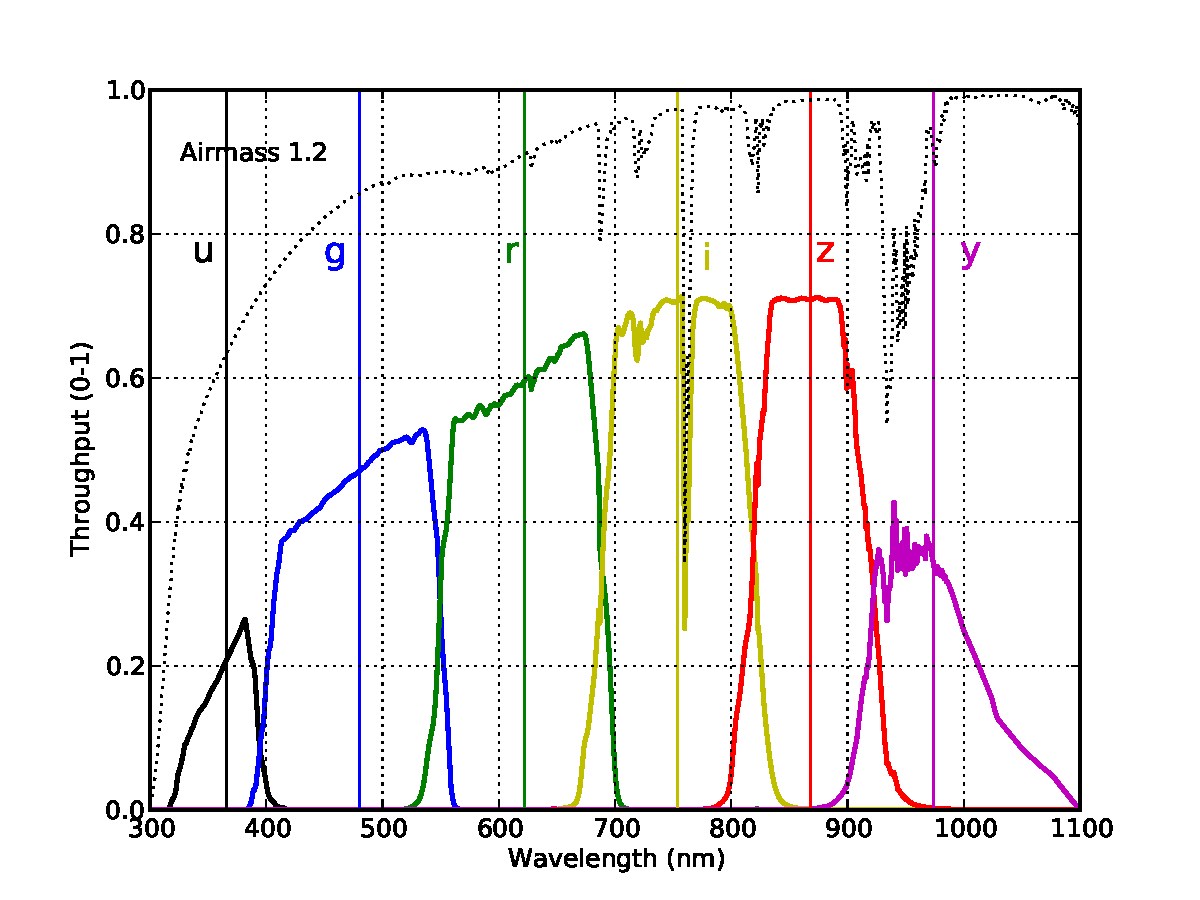
\includegraphics[width=5in]{filters}
\end{figure}


\section{Improvements in photometric accuracy}

To conduct science with the catalogs from LSST, the natural magnitudes, $m_b^{nat}$, for each astronomical object in
each visit must obviously be recorded, resulting in approximately
$2\times10^{13}$ measurements. However, in order to permit scientists
to generate higher precision photometry for objects with known SEDs
(which are likely to be different than the SEDs LSST used to create
those $m_b^{nat}$ measurements),
$\phi_b^{visit}(\lambda,alt,az,x,y,t)$ and the zeropoint offset from
the self-calibration procedure must also be available. With these
additional pieces of information, scientists can generate more precise
$\delta k(alt,az,x,y,SED,t)$ corrections to $m_b^{nat}$.

TODO : need to look at the differences in $m_b^{obs}$ resulting from
using a completely flat (within each filter) SED, an actual star or
galaxy or SN SED, a flat SED that has been 'tilted' to have the right
color (i.e. straight line SED, slope!=0) in various cases of
$\phi_b$. This has bearing on what type of SED LSST should use in
general (probably flat) and what must be used to generate input
magnitudes for the self-cal. Also has bearing on what resolution
$\phi_b$ must be recorded with.   (also, while doing this : how much
scatter is introduced to $m_b^{nat}$ due to using the wrong SED? -
evaluate difference between flat and true SED corrected magnitudes under range of different
$\phi_b$)  ($m_b^{nat}$ = standardized $\phi_b$, $m_b^{obs}$ =
observed $\phi$). 

CREATE FIGURE: the likely magnitude of these corrections (part of the output
of the TODO above)

Data management could record a full $\phi_b^{visit}(\lambda,alt,az,x,y,t)$ value
for every object in every visit, where the resolution on
$\phi(\lambda)$ will need to be about 0.5~nm.  It should also be possible
for data management to simply record the full narrow band flats field
set, the synthetic flat field applied to the image, 
the interpolated components for the atmosphere (approximately 6
parameters per visit), and the zeropoint applied to each patch
(approximately 369 per visit). Together with provenance information on
how each of these was used to generate the observational corrections,
it would be possible to regenerate a higher precision $m_b^{nat}$. 


%\section{Comparison of standard calibration and SDSS ubercal (as
% approximation for this method)}


%\section{Thermal IR Camera}
%possibility to generate measurement of shape of cloud structure over
%field of view (could function as prior for self-calibration)

%if cloud structure found to vary on scales smaller than length between
%calibration stars (or minimum scale possible to correct with
%self-calib), then thermal IR camera would enable generation of
%these corrections

%may provide useful SDQA data (especially for alerts/nightly data
%stream)


\end{document}
